\section{Motivation}

\subsection[Problem Presentation]{Problem Presentation}
\begin{frame}
  \frametitle{Problem Presentation}
  
  \begin{itemize}
  \item Erlang supports records with named fields
  \item Operations:
    \begin{itemize}
    \item Create new instance (possibly using default values)
    \item Retrieve a specific field
    \item Pattern match on multiple fields
    \item Create a new record from an existing one, updating some fields
    \end{itemize}
  \item Records are often used to represent ``state''
  \end{itemize}
\end{frame}

\begin{frame}
  \frametitle{Problem Presentation}
  \begin{itemize}
  \item Records are implemented internally with tuples
  \item Erlang passes terms by reference...
    \pause
  \item ... except when it doesn't!
    \begin{itemize}
    \item Spawning a new process
    \item Sending a message to a process
    \item Storing a term in an Elang Term Storage table
    \item ... pretty printing a term to stdout!
    \end{itemize}
    \pause
  \item In these cases the term is copied to the heap of the destination
    process
  \item Copying large terms can take some time and can also result in terms of
    bigger size in the destination (in the current version, copying destroys
    sharing within a term)
  \end{itemize}
\end{frame}

\begin{frame}
  \frametitle{Problem Presentation}
  
  \begin{figure}
    \centering
    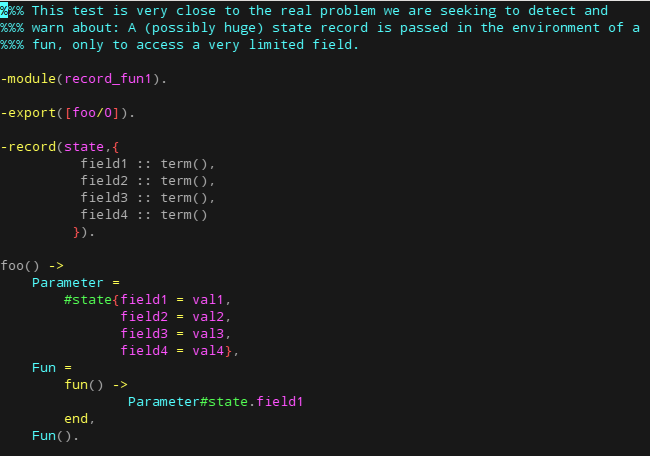
\includegraphics[scale=0.45]{../figures/problem_introduction}
  \end{figure}
  
\end{frame}

\begin{frame}
  \frametitle{Solution Introduction}
  
  \begin{itemize}
  \item The Recorder Analyzer:
    \begin{itemize}
    \item Detect cases where an argument is treated as a record but not all
      fields are accessed
    \item Automatic optimization is not always safe $\to$ emit warnings instead
    \item Operates on single functions (named or anonymous)
    \end{itemize}
  \item Recorder characteristics
    \begin{itemize}
    \item Correctness
    \item Accuracy
    \item User friendliness
    \item Extensibility
    \end{itemize}
  \end{itemize}
  
\end{frame}
